\documentclass{article}
\usepackage{graphicx} % Required for inserting images

\title{CTA200 Assignment 3 Figures}
\author{Andrew Li | 1006675625 | andrewp.li@mail.utoronto.ca}
\date{May 9, 2023}

\usepackage{amsfonts}
\usepackage{amsmath}
\usepackage{url}
\usepackage{graphicx}
\usepackage{float}
\usepackage{listings}

\usepackage{geometry}
 \geometry{
 left=25mm,
 right=25mm,
 top=25mm,
 bottom=25mm,
 }

\usepackage{physics}
\usepackage{verbatim}
\usepackage{wrapfig}
\usepackage{hyperref}
\usepackage{natbib}

\usepackage{minted}
\usepackage{xcolor}
\definecolor{LightGray}{gray}{0.9}

\bibliographystyle{aasjournal}

\begin{document}

\maketitle

\begin{figure}[H]
\begin{center}
    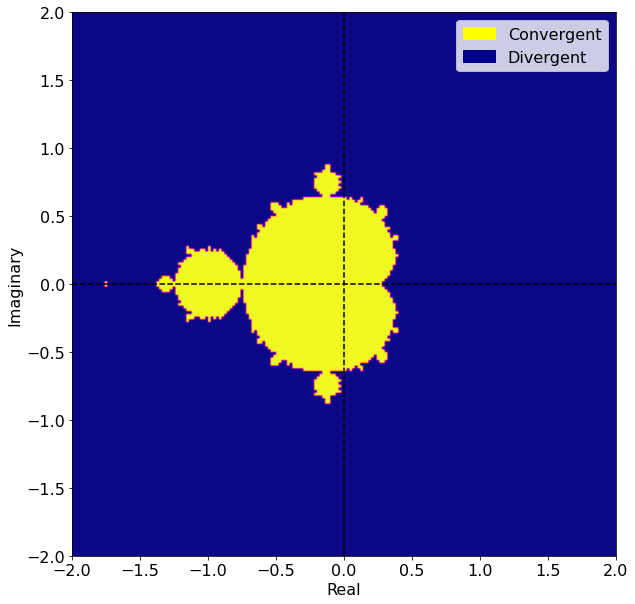
\includegraphics[width=0.45\textwidth]{figures/mandelbrot 1.png}
    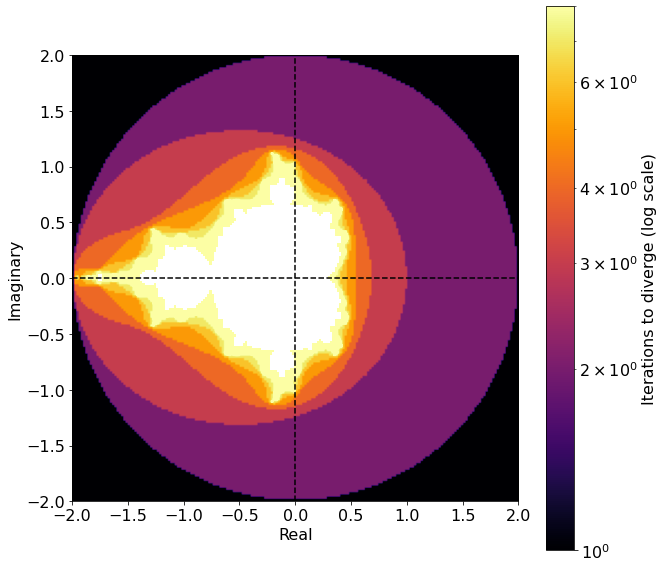
\includegraphics[width=0.5\textwidth]{figures/mandelbrot 2.png}
\end{center}
\vspace{-2em}
    \caption{The results of \texttt{complex\_iterate(N=200,z0=0,max\_iter=1000)}. Left: The convergent values (\texttt{np.nan}) are shown in yellow, and the divergent values are shown in blue. Right: The convergent values are now shown in white, and the divergent values are shown based on the iteration at which it diverged in accordance to the colorbar. Note the logarithmic scale.}
    \label{fig:1}
\end{figure}

\begin{figure}[H]
\begin{center}
    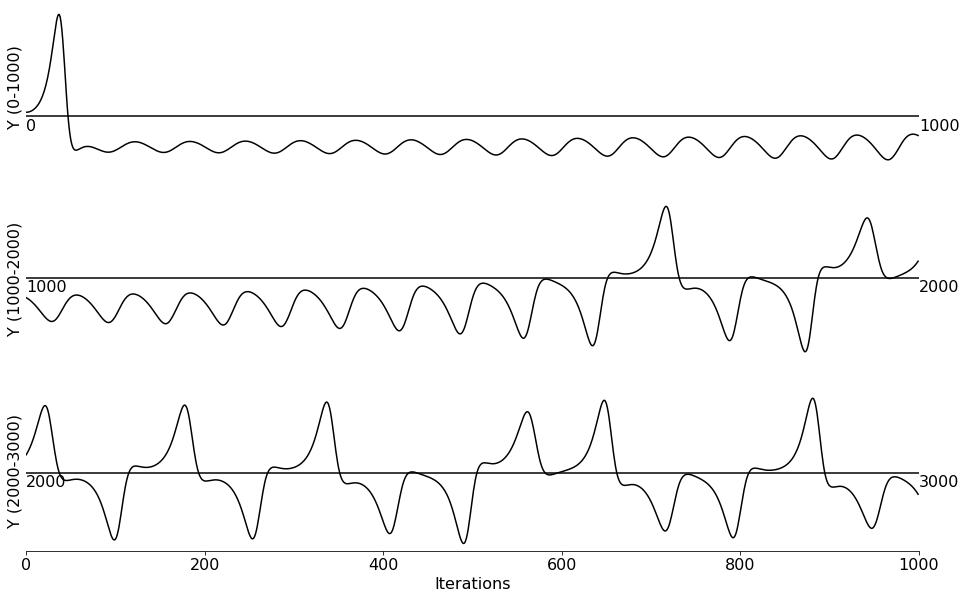
\includegraphics[width=\textwidth]{figures/lorenz 1.png}
\end{center}
\vspace{-2em}
    \caption{$Y$ over the first 3000 iterations ($\Delta t=0.01$). The first 1000 are on the top, 1000-2000 are in the middle, and 2000-3000 are on the bottom. The $y$-axis are the relative $Y$ values.}
    \label{fig:2}
\end{figure}

\begin{figure}[H]
\begin{center}
    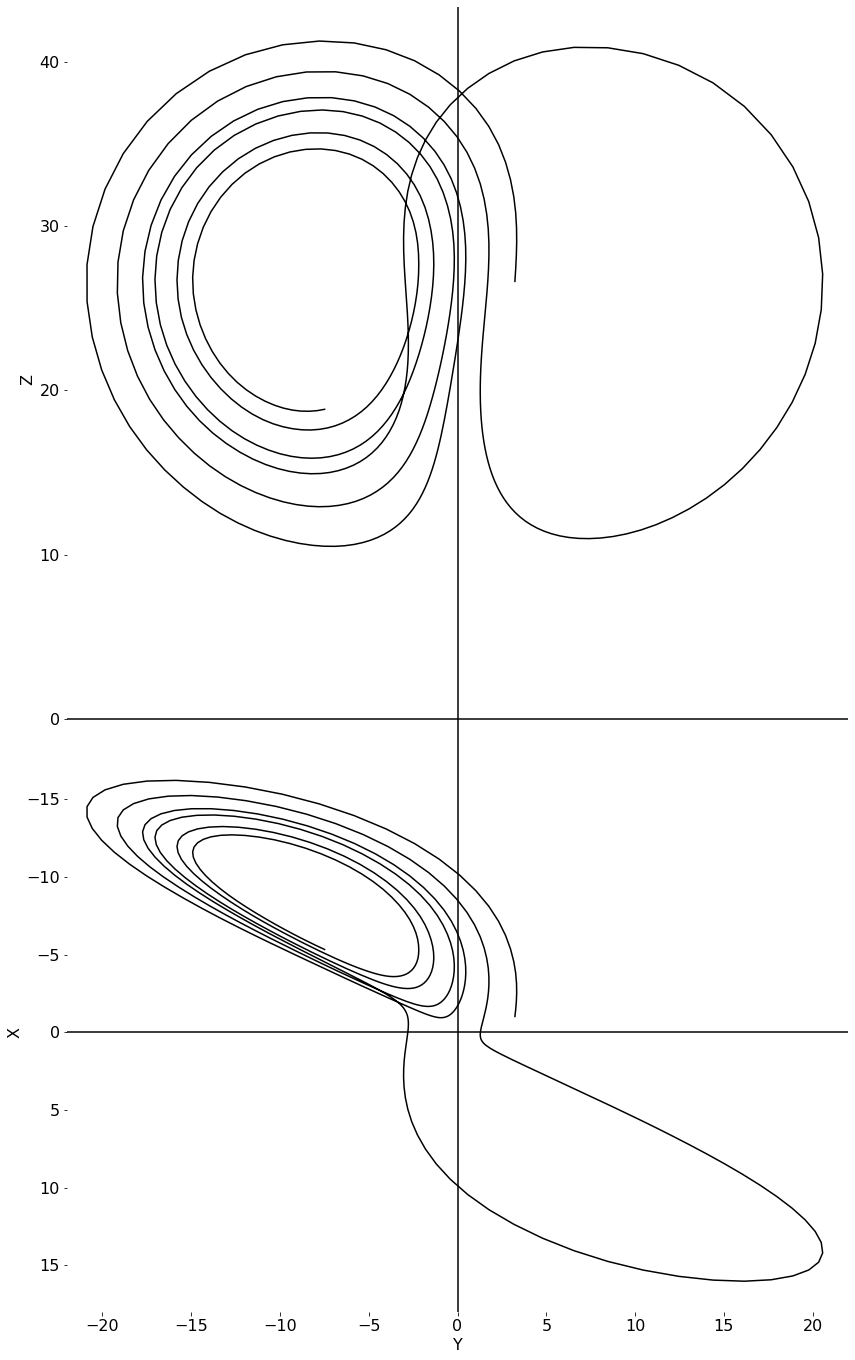
\includegraphics[width=0.8\textwidth]{figures/lorenz 2.png}
\end{center}
\vspace{-2em}
    \caption{$Z$-$Y$ plot (above) and $X$-$Y$ (below) plot over iterations 1400-1900.}
    \label{fig:3}
\end{figure}

\begin{figure}[H]
\begin{center}
    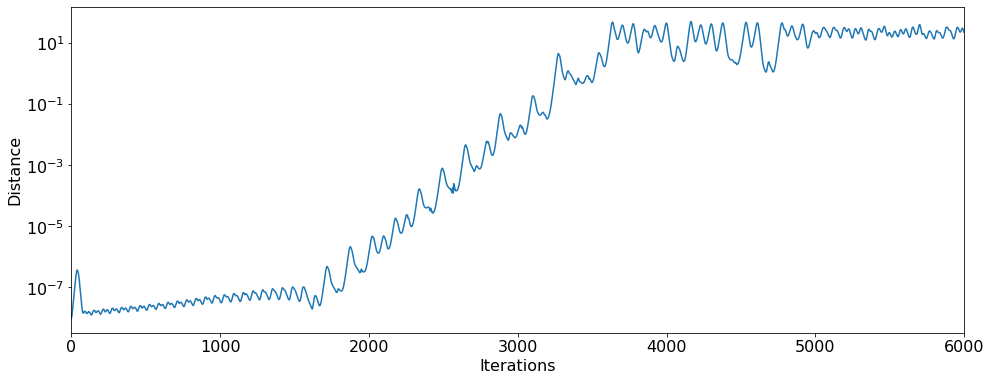
\includegraphics[width=\textwidth]{figures/diff.png}
\end{center}
\vspace{-2em}
    \caption{Semi-log plot of the differences betewen using $W_0$ and $W_0'$.}
    \label{fig:4}
\end{figure}

\end{document}
